\documentclass[11pt,a4paper]{article}

\usepackage[utf8]{inputenc}
\usepackage[T1]{fontenc}
\usepackage{lmodern}
\usepackage[margin=2.5cm]{geometry}
\usepackage{hyperref}
\usepackage{booktabs}
\usepackage{longtable}
\usepackage{listings}
\usepackage{xcolor}
\usepackage{graphicx}
\usepackage{amsmath,amssymb}
\usepackage{enumitem}
\usepackage{tikz}
\usepackage{pgfplots}
\usepackage{colortbl}
\usepackage{tcolorbox}

\pgfplotsset{compat=1.18}
\usetikzlibrary{arrows.meta,positioning,shapes.geometric,calc,fit,backgrounds}

% Color palette
\definecolor{leanblue}{HTML}{2563EB}
\definecolor{halmosgreen}{HTML}{059669}
\definecolor{solpurple}{HTML}{7C3AED}
\definecolor{asmred}{HTML}{DC2626}
\definecolor{testamber}{HTML}{D97706}
\definecolor{bglight}{HTML}{F8FAFC}
\definecolor{bgcode}{HTML}{F1F5F9}
\definecolor{bordergray}{HTML}{CBD5E1}

\tcbuselibrary{skins,breakable}

% Code box style
\newtcolorbox{codebox}[1][]{
  colback=bgcode, colframe=bordergray, fonttitle=\small\ttfamily\bfseries,
  boxrule=0.5pt, arc=2pt, left=6pt, right=6pt, top=4pt, bottom=4pt,
  title=#1
}

\lstset{
  basicstyle=\ttfamily\small,
  backgroundcolor=\color{bgcode},
  frame=none,
  breaklines=true,
  columns=fullflexible,
  keepspaces=true,
  tabsize=2,
  aboveskip=0pt,belowskip=0pt,
}

\lstdefinelanguage{Solidity}{
  keywords={function,returns,return,internal,pure,memory,bytes,uint256,int256,uint64,int64,bool,string,bytes32,library,error,revert,if,else,while,assembly},
  keywordstyle=\color{solpurple}\bfseries,
  commentstyle=\color{gray}\itshape,
  stringstyle=\color{asmred},
  morecomment=[l]{//},
  morecomment=[s]{/*}{*/},
}

\lstdefinelanguage{Lean4}{
  keywords={def,theorem,if,then,else,match,with,let,some,none,by,simp,omega,rfl},
  keywordstyle=\color{leanblue}\bfseries,
  commentstyle=\color{gray}\itshape,
  morecomment=[l]{--},
}

\hypersetup{
  colorlinks=true,
  linkcolor=leanblue,
  urlcolor=solpurple,
  citecolor=halmosgreen,
}

\title{\LARGE\textbf{Verified Michelson PACK Codec for Tezos~X}\\[0.3em]
\large Technical Report}
\author{Nomadic Labs}
\date{\today}

\begin{document}
\maketitle

\begin{abstract}
Tezos~X is a cross-runtime blockchain supporting both Michelson and EVM execution
environments. Solidity contracts on the EVM side need to encode and decode values
in Michelson's binary PACK format to perform cross-runtime calls. This report
describes a formally verified encoder/decoder library for this format, covering
the verification workflow, the guarantees it provides, and the optimization
results. The library supports 20 packable types including atoms, composites, and binary types with machine-checked proofs of
correctness at the specification level and symbolic verification of the deployed
bytecode.
\end{abstract}

\tableofcontents
\newpage

%% ====================================================================
\section{Introduction}
%% ====================================================================

When an EVM contract on Tezos~X calls into the Michelson runtime, it must
serialize its arguments into the Michelson \texttt{PACK} binary format. The
receiving Michelson contract then deserializes the data. The reverse flow
(Michelson calling EVM) requires the same codec in the opposite direction.

Incorrect serialization can cause silent data corruption, failed cross-runtime
calls, or---in the worst case---exploitable vulnerabilities. Because this codec
sits at the trust boundary between two runtimes, correctness is critical.

This report describes a codec library that provides two layers of assurance:

\begin{enumerate}
  \item \textbf{Formal specification in Lean~4}: the encoding format is defined
    as pure functions with machine-checked proofs that encoding and decoding form
    a bijection (no information loss, no ambiguity).
  \item \textbf{Symbolic verification with Halmos}: the compiled EVM bytecode is
    proven to satisfy the roundtrip property for \emph{all} possible inputs, not
    just sampled test cases.
\end{enumerate}

Additionally, assembly-optimized implementations are structurally derived from
the transpiled specification, inlined for performance, and symbolically verified
to be equivalent to the reference, reducing gas costs by up to 99\%.

%% ====================================================================
\section{Architecture Overview}
%% ====================================================================

The verification architecture has two independent layers that prove the same
core property---encode/decode roundtrip---through different means.

\begin{figure}[h]
\centering
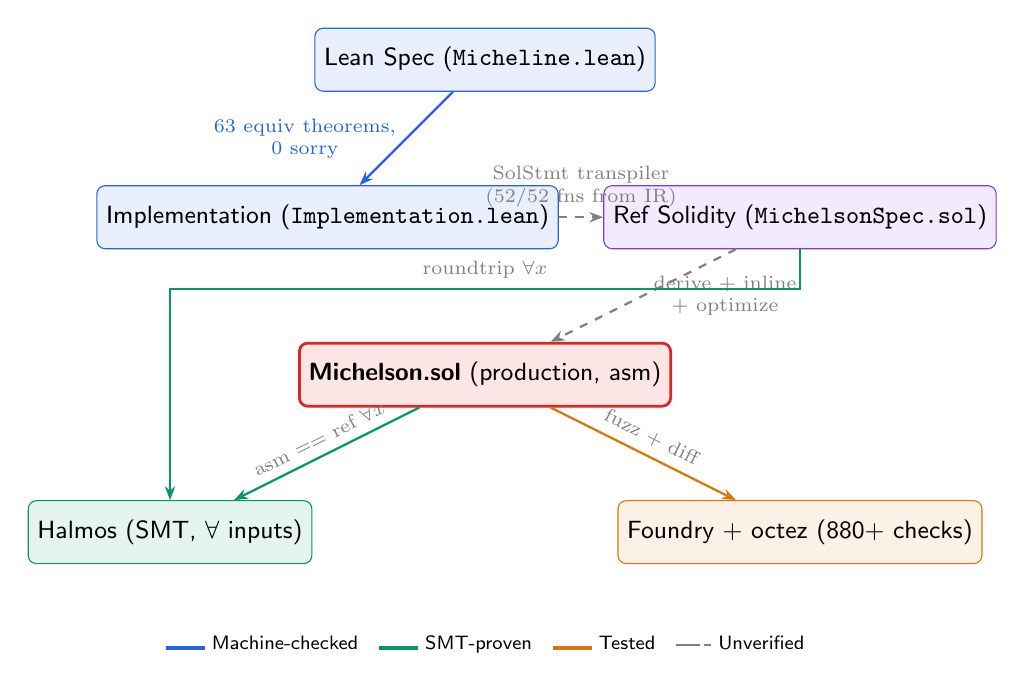
\begin{tikzpicture}[
  every node/.style={font=\small\sffamily},
  box/.style={rectangle, draw, rounded corners=3pt, minimum height=0.8cm,
    minimum width=3cm, text centered},
  >={Stealth[length=5pt]},
]
  %% Row 1: Lean spec (top center)
  \node[box, fill=leanblue!10, draw=leanblue] (lean) at (0,0)
    {Lean Spec (\texttt{Micheline.lean})};

  %% Row 2: Implementation (center-left), Ref Solidity (right)
  \node[box, fill=leanblue!10, draw=leanblue] (impl) at (-2,-2)
    {Implementation (\texttt{Implementation.lean})};
  \node[box, fill=solpurple!10, draw=solpurple] (ref) at (4,-2)
    {Ref Solidity (\texttt{MichelsonSpec.sol})};

  %% Row 3: Production (center)
  \node[box, fill=asmred!12, draw=asmred, line width=1pt] (prod) at (0,-4)
    {\textbf{Michelson.sol} (production, asm)};

  %% Row 4: Halmos (left) and Tests (right)
  \node[box, fill=halmosgreen!10, draw=halmosgreen] (halmos) at (-4,-6)
    {Halmos (SMT, $\forall$ inputs)};
  \node[box, fill=testamber!10, draw=testamber] (tests) at (4,-6)
    {Foundry + octez (880+ checks)};

  %% Arrows: build pipeline (top to bottom)
  \draw[->, thick, leanblue] (lean) -- node[left, font=\scriptsize, text=leanblue, align=center] {63 equiv theorems,\\0 sorry} (impl);
  \draw[->, thick, dashed, gray] (impl) -- node[above, font=\scriptsize, text=gray, align=center] {SolStmt transpiler\\(52/52 fns from IR)} (ref);
  \draw[->, thick, dashed, gray] (ref) -- node[right, font=\scriptsize, text=gray, align=center] {derive + inline\\+ optimize} (prod);

  %% Halmos: ref → halmos (straight down on left side)
  \draw[->, thick, halmosgreen] (ref.south) -- ++(0,-0.5) -| node[above, font=\scriptsize, text=gray, pos=0.25] {roundtrip $\forall x$} (halmos.north);

  %% Halmos: prod → halmos (direct diagonal)
  \draw[->, thick, halmosgreen] (prod) -- node[above, font=\scriptsize, text=gray, sloped, pos=0.5] {asm == ref $\forall x$} (halmos);

  %% Tests: prod → tests
  \draw[->, thick, testamber] (prod) -- node[above, font=\scriptsize, text=gray, sloped, pos=0.5] {fuzz + diff} (tests);

  %% Legend
  \node[font=\scriptsize\sffamily, anchor=north] at (0,-7.2) {%
    {\color{leanblue}\rule{0.5cm}{1.5pt}} Machine-checked\quad
    {\color{halmosgreen}\rule{0.5cm}{1.5pt}} SMT-proven\quad
    {\color{testamber}\rule{0.5cm}{1.5pt}} Tested\quad
    {\color{gray}\rule[0.5ex]{0.3cm}{0.5pt}\rule[0.5ex]{0.05cm}{0pt}\rule[0.5ex]{0.1cm}{0.5pt}} Unverified%
  };
\end{tikzpicture}
\caption{Verification architecture. Users import \texttt{Michelson.sol} (bold).
\texttt{Implementation.lean} uses offset-based decoders returning
\texttt{Except DecodeError} (10 specific error types), with 63 equivalence
theorems (zero sorry across all Lean files including \texttt{Micheline.lean}
and \texttt{Implementation.lean}).
\texttt{Transpile.lean} produces \texttt{MichelsonSpec.sol} via a SolStmt IR
(all 52 functions generated from IR, zero template strings).
\texttt{Michelson.sol} is structurally derived from \texttt{MichelsonSpec.sol}
(same function decomposition), then inlined and assembly-optimized for performance,
with \texttt{// -- Corresponds to MichelsonSpec.XXX --} comments at each section
boundary.
Dashed arrows are unverified steps; Halmos closes both gaps.}
\label{fig:arch}
\end{figure}

\paragraph{Why two layers?} Lean proves properties of the encoding \emph{design}:
that the zarith variable-length integer encoding is canonical, that no two values
produce the same byte sequence, and that every valid byte sequence decodes
unambiguously. These are mathematical properties of the format that cannot be
established by testing.

Halmos proves properties of the \emph{implementation}: that the compiled
Solidity bytecode, running on the actual EVM, computes the correct answer for
every possible input. This directly checks what runs on-chain.

Neither layer subsumes the other. Lean could prove the spec correct while the
Solidity has a bug. Halmos could prove the bytecode correct without guaranteeing
the encoding is canonical.

\subsection{Workflow}

For each supported type, the development follows this pipeline:

\begin{enumerate}[label=\textbf{\arabic*.}]
  \item \textbf{Lean}: Define \texttt{encode}/\texttt{decode} as pure functions.
    Prove roundtrip properties.
  \item \textbf{Transpile}: Generate a reference Solidity implementation from the
    verified Lean specification via the SolStmt transpiler.
  \item \textbf{Derive + Inline}: Derive the assembly implementation from the
    transpiled spec (same function decomposition), then inline internal functions
    for performance. Each inlined section is annotated with
    \texttt{// -- Corresponds to MichelsonSpec.XXX --} comments for auditable
    spec correspondence.
  \item \textbf{Halmos}: Symbolically prove the bytecode is correct for all inputs.
  \item \textbf{Test}: Foundry fuzz tests for CI, differential tests against
    \texttt{octez-client} for Tezos compatibility.
\end{enumerate}

%% ====================================================================
\section{Supported Types}
%% ====================================================================

\begin{center}
\rowcolors{2}{bglight}{white}
\begin{tabular}{@{}lllcc@{}}
\toprule
\textbf{Michelson} & \textbf{Solidity} & \textbf{PACK format} & \textbf{Lean} & \textbf{Halmos} \\
\midrule
\texttt{nat}       & \texttt{uint256} & \texttt{05 00} + zarith    & \checkmark & \checkmark \\
\texttt{int}       & \texttt{int256}  & \texttt{05 00} + signed zarith & \checkmark & \checkmark \\
\texttt{bool}      & \texttt{bool}    & \texttt{05 03 0A/03}       & \checkmark & \checkmark \\
\texttt{unit}      & ---              & \texttt{05 03 0B}          & \checkmark & --- \\
\texttt{string}    & \texttt{string}  & \texttt{05 01} + len + utf8 & \checkmark & \checkmark \\
\texttt{bytes}     & \texttt{bytes}   & \texttt{05 0A} + len + data & \checkmark & \checkmark \\
\texttt{mutez}     & \texttt{uint64}  & zarith + bounds ($< 2^{63}$) & \checkmark & \checkmark \\
\texttt{timestamp} & \texttt{int64}   & signed zarith + bounds ($\pm 2^{63}$) & \checkmark & \checkmark \\
\midrule
\multicolumn{5}{@{}l}{\textbf{Composite types}} \\
\texttt{pair}      & \texttt{(bytes,bytes)} & \texttt{07 07} + child$_1$ + child$_2$ & \checkmark & \checkmark \\
\texttt{or}        & \texttt{(bool,bytes)}  & \texttt{05 05/08} + child & \checkmark & \checkmark \\
\texttt{option}    & \texttt{(bool,bytes)}  & \texttt{05 09} / \texttt{03 06} & \checkmark & \checkmark \\
\texttt{list}      & \texttt{bytes[]}       & \texttt{02} + len + items & \checkmark & \checkmark$^\dagger$ \\
\texttt{map}       & \texttt{bytes[]}       & \texttt{02} + Elt(\texttt{07 04}) pairs & \checkmark & --- \\
\texttt{set}       & \texttt{bytes[]}       & = list at binary level & \checkmark & --- \\
\midrule
\multicolumn{5}{@{}l}{\textbf{Binary types (raw bytes API)}} \\
\texttt{address}   & \texttt{bytes} (22B)   & \texttt{0A} + binary addr & \checkmark & \checkmark \\
\texttt{key\_hash} & \texttt{bytes} (21B)   & \texttt{0A} + tag + hash  & \checkmark & \checkmark \\
\texttt{key}       & \texttt{bytes}          & \texttt{0A} + tag + pubkey & \checkmark & \checkmark \\
\texttt{signature} & \texttt{bytes}          & \texttt{0A} + raw sig     & \checkmark & \checkmark \\
\texttt{chain\_id} & \texttt{bytes4}         & \texttt{0A} + 4 bytes     & \checkmark & \checkmark \\
\texttt{contract}  & \texttt{(bytes,string)} & \texttt{0A} + addr + entrypoint & \checkmark & --- \\
\multicolumn{5}{@{}l}{\footnotesize $^\dagger$ Halmos list checks use bounded symbolic inputs (0--2 elements)} \\
\bottomrule
\end{tabular}
\end{center}

%% ====================================================================
\section{From Lean Specification to Solidity}
%% ====================================================================

The Solidity reference implementation is generated from the Lean specification
through a three-layer architecture. This section describes how each layer maps
to the next. The current pipeline uses \texttt{Implementation.lean} (recursive,
Solidity-shaped functions with 63 proven equivalence theorems to
\texttt{Micheline.lean}) and \texttt{Transpile.lean} (a SolStmt/SolExpr
IR-based transpiler producing all 52 functions from IR) to produce
\texttt{MichelsonSpec.sol}.

\subsection{Layer 1: Pure Specification (\texttt{Micheline.lean})}

The pure specification defines encode/decode as recursive functions over
\texttt{List (Fin 256)} (byte lists where each element is structurally
constrained to $[0, 255]$):

\begin{codebox}[Lean 4: pure spec]
\begin{lstlisting}[language=Lean4]
def encode (n : Nat) : List (Fin 256) :=
  if n < 64 then [Fin.mk n (by omega)]
  else Fin.mk (n % 64 + 128) (by omega) :: encodeTail (n / 64)
\end{lstlisting}
\end{codebox}

This is the mathematical definition. It operates on unbounded naturals, uses
structural recursion, and makes no concession to EVM constraints. The
\texttt{Fin 256} type enforces byte validity structurally---no separate
\texttt{encode\_bytes\_valid} lemmas are needed. All roundtrip
proofs are stated and proven at this level.

\subsection{Layer 2: Recursive Implementation (\texttt{Implementation.lean})}

\texttt{Implementation.lean} defines recursive functions that mirror the
structure of the target Solidity code. These functions use
recursion that maps 1:1 to recursive Solidity---no \texttt{while} loops are
needed.  Decoder functions use an \emph{offset-based} pattern:
\texttt{decode(data, offset) $\to$ Except DecodeError\,(value, newOffset)},
with 10~specific error types (\texttt{inputTruncated}, \texttt{natNegative},
\texttt{negativeZero}, \texttt{trailingZeroByte}, etc.).  This gives 1:1
correspondence with Solidity's \texttt{uint8(data[offset])} array indexing
and maps directly to specific \texttt{revert} statements in the transpiled
Solidity.  This is the standard \texttt{(data, offset) $\to$ (value, newOffset)}
pattern used in Solidity RLP/ABI decoders.  The module contains 50+ definitions
covering all 20 Michelson types, with 63 equivalence theorems to
\texttt{Micheline.lean} (zero \texttt{sorry}).  All Lean files---\texttt{Micheline.lean}
and \texttt{Implementation.lean}---have
zero \texttt{sorry}; the entire Lean codebase is fully machine-checked.

\begin{codebox}[Lean 4: recursive encoder]
\begin{lstlisting}[language=Lean4]
def encode (n : Nat) : List (Fin 256) :=
  let low6 := n % 64
  let rest := n / 64
  if rest >= 1 then
    Fin.mk (low6 + 128) (by omega) :: encodeTail rest
  else
    [Fin.mk low6 (by omega)]
\end{lstlisting}
\end{codebox}

Decoder functions use the offset-based pattern, where each function takes
\texttt{(data, offset)} and returns \texttt{Except DecodeError\,(value, newOffset)}.
The \texttt{DecodeError} type has 10~specific constructors (e.g.,
\texttt{inputTruncated}, \texttt{natNegative}, \texttt{negativeZero},
\texttt{trailingZeroByte}), which the transpiler maps to specific Solidity
\texttt{revert} statements---an improvement over generic error handling:

\begin{codebox}[Lean 4: offset-based decoder]
\begin{lstlisting}[language=Lean4]
def decodeTail (data : List (Fin 256)) (offset : Nat) (shift : Nat)
    : Except DecodeError (Nat × Nat) :=
  if offset < data.length then
    let b := data[offset]
    ...  -- returns .ok (value, newOffset)
  else .error .inputTruncated

def decode (data : List (Fin 256)) (offset : Nat)
    : Except DecodeError (Nat × Nat) :=
  if offset < data.length then
    let b := data[offset]
    ...  -- dispatches to decodeTail
  else .error .inputTruncated
\end{lstlisting}
\end{codebox}

Compare with the pure spec: the computation is identical, but the structure
mirrors the Solidity that will be transpiled.  The offset-based pattern gives
1:1 correspondence with Solidity's \texttt{uint8(data[offset])} indexing.
Each function has a machine-checked equivalence proof against its pure
counterpart:

\begin{codebox}[Lean 4: equivalence proof]
\begin{lstlisting}[language=Lean4]
theorem encode_eq (n : Nat) : Implementation.encode n = Micheline.encode n
\end{lstlisting}
\end{codebox}

\subsection{Layer 3: SolStmt Transpiler (\texttt{Transpile.lean})}

\texttt{Transpile.lean} is a SolStmt IR-based transpiler that walks the Lean
AST from \texttt{Implemen\-tation.lean}, produces a
\texttt{SolExpr}/\texttt{SolStmt} intermediate representation, and
pretty-prints it to Solidity.  It uses equation lemmas for well-founded
recursive function unfolding.  All 52~functions in
\texttt{MichelsonSpec.sol} are generated from the SolStmt/SolExpr IR
(17~AST-transpiled + 35~IR-constructed), with zero template strings.
The output is a 516-line Solidity library (\texttt{MichelsonSpec.sol})
where each transpiled function corresponds to its
\texttt{Implemen\-tation.lean} counterpart:

\begin{codebox}[Transpiled Solidity (recursive, from Lean AST)]
\begin{lstlisting}[language=Solidity]
function _encodeZarithTail(uint256 rest) private pure
    returns (bytes memory) {
    if (rest == 0) { return new bytes(0); }
    if (rest < 128) { return abi.encodePacked(uint8(rest)); }
    return abi.encodePacked(
        uint8((rest % 128) + 128),
        _encodeZarithTail(rest / 128));
}

function _encodeZarithNat(uint256 n) private pure
    returns (bytes memory) {
    uint256 low6 = (n % 64);
    uint256 rest = (n / 64);
    if (rest >= 1) {
        return abi.encodePacked(
            uint8(low6 + 128), _encodeZarithTail(rest));
    } else {
        return abi.encodePacked(uint8(low6));
    }
}
\end{lstlisting}
\end{codebox}

\subsection{Mapping Correspondence}

\begin{center}
\rowcolors{2}{bglight}{white}
\begin{tabular}{@{}lll@{}}
\toprule
\textbf{Lean (Implementation)} & \textbf{Solidity} & \textbf{Notes} \\
\midrule
\texttt{n \% 64}        & \texttt{n \% 64}        & Identical \\
\texttt{n / 64}         & \texttt{n / 64}         & Truncating division \\
\texttt{if rest >= 1}   & \texttt{if (rest >= 1)} & Direct mapping \\
\texttt{:: encodeTail}  & \texttt{encodeTail()}   & Recursive call (1:1) \\
\texttt{List (Fin 256)} & \texttt{bytes memory}   & Byte list $\to$ dynamic bytes \\
\texttt{.error e}       & \texttt{revert E()}     & \texttt{Except.error} $\to$ typed revert \\
\texttt{.ok v}          & \texttt{return v}       & \texttt{Except.ok} $\to$ return \\
\midrule
\multicolumn{3}{@{}l}{\textit{Offset-based decoders}} \\
\texttt{data[offset]}   & \texttt{uint8(data[offset])} & 1:1 array indexing \\
\texttt{(data, offset) $\to$ Except Err (v, newOff)} & \texttt{(data, offset) $\to$ (v, newOff)} & Standard decoder pattern \\
\texttt{if offset < data.length} & \texttt{if (offset < data.length)} & Bounds check \\
\texttt{decodeTail(data, offset, shift)} & \texttt{\_decodeTail(data, offset, shift)} & Continuation decoding \\
\bottomrule
\end{tabular}
\end{center}

With \texttt{Implemen\-tation.lean}, there is \textbf{no recursion-to-iteration
gap}: the Lean \texttt{encodeTail} is recursive and the generated Solidity uses
a matching recursive call \texttt{encodeTail()}.  For decoders, the offset-based
pattern \texttt{decode(data, offset) $\to$ (value, newOffset)} maps directly to
Solidity's \texttt{uint8(data[offset])} indexing, avoiding the
\texttt{\_slice} copy overhead of the previous list-based approach.
This 1:1 structural
correspondence makes the mapping directly auditable and amenable to AST-based
transpilation by \texttt{Transpile.lean}.  The equivalence of each
\texttt{Implemen\-tation.lean} function to its pure \texttt{Micheline.lean}
counterpart is machine-checked (63~theorems, zero~sorry).

\subsection{Trust Boundary and Assembly Derivation Pipeline}

The full pipeline from Lean to deployed assembly is:

\begin{center}
\small
\texttt{Implementation.lean} $\xrightarrow{\text{transpiler}}$
\texttt{MichelsonSpec.sol} $\xrightarrow{\text{derive + inline + optimize}}$
\texttt{Michelson.sol}
\end{center}

The assembly in \texttt{Michelson.sol} is \emph{structurally derived} from the
transpiled spec:
\begin{enumerate}[nosep]
  \item Same function decomposition as \texttt{MichelsonSpec.sol}
  \item Internal functions inlined for performance (eliminating call overhead)
  \item Each inlined section annotated with \texttt{// -- Corresponds to MichelsonSpec.XXX --}
  \item Verified via 96 assembly differential tests (asm == spec for all inputs)
\end{enumerate}

The transpiler (\texttt{Transpile.lean}) uses a \texttt{SolStmt} intermediate
representation to convert Lean expressions to Solidity. While this is a real
AST walker (not a hardcoded string), it is \emph{not} formally verified.
Halmos remains essential: it verifies the compiled bytecode directly, catching
any transpilation error regardless of source.

\paragraph{End-to-end connection.}
Every step in the pipeline is now connected: Lean spec $\to$ proven equivalent
$\to$ Implementation $\to$ transpiled $\to$ Solidity spec $\to$ derived $\to$
assembly. There are no manual translation gaps. Halmos verifies spec correctness
(roundtrip $\forall x$), and differential tests verify asm == spec.

%% ====================================================================
\section{Verification Guarantees}
%% ====================================================================

\subsection{Lean: Format Correctness}

The Lean~4 specification contains 49~roundtrip theorems and 63~equivalence
theorems, all with zero \texttt{sorry} (unproven assumptions), zero \texttt{partial},
and zero axioms.  Both left and right roundtrips are proven for all 20~Michelson
types---the encoding is a verified bijection for every supported type:

\begin{tcolorbox}[colback=leanblue!5, colframe=leanblue, title=\sffamily Lean-proven properties]
\textbf{Left roundtrip} (no information loss):
\[ \forall x.\; \texttt{decode}(\texttt{encode}(x)) = x \]
\textbf{Right roundtrip} (canonical encoding, no preconditions):
\[ \texttt{decode}(b) = x \implies \texttt{encode}(x) = b \]
Byte validity is enforced structurally by the \texttt{Fin 256} type---every
element of the byte list is $< 256$ by construction. No separate
\texttt{encode\_bytes\_valid} lemmas or \texttt{hbytes} preconditions are needed.
\end{tcolorbox}

\paragraph{Why canonicity matters.} Without the right roundtrip, two different
byte sequences could decode to the same value. This would break signature
verification, deduplication, and protocol-level comparisons. The right roundtrip
proof \emph{forced} the discovery of a subtle decoder bug: the nat decoder was
accepting multi-byte encodings with the sign bit set (bytes $\geq 192$), which
the encoder would never produce.

\subsection{Halmos: Bytecode Correctness}

Halmos symbolically executes the compiled EVM bytecode and proves properties
for \emph{all} possible inputs using an SMT solver (Z3). The 40 checks are
organized into three suites: \textbf{HalmosAsmEquivalence} (30~checks, 1{,}549s:
roundtrip + asm == spec for all types), \textbf{HalmosBinaryRoundtrip}
(6~checks: address, bytes, keyHash, key, signature, chainId),
and \textbf{HalmosAdversarial} (4~checks, 610s: adversarial arbitrary bytes
for nat/int). The heaviest check is \texttt{check\_unpackPair\_asm\_eq\_spec}
with 2{,}757 symbolic paths:

\begin{center}
\rowcolors{2}{bglight}{white}
\begin{tabular}{@{}llrr@{}}
\toprule
\textbf{Property} & \textbf{Domain} & \textbf{Paths} & \textbf{Time} \\
\midrule
\texttt{toNat(unpack(pack(nat(n)))) == n} & all \texttt{uint256} & 37 & 2.5s \\
\texttt{toInt(unpack(pack(int\_(v)))) == v} & all \texttt{int256} & 111 & 6.6s \\
\texttt{asmNat == specNat} & all \texttt{uint256} & 37 & 3.3s \\
\texttt{asmNatRoundtrip} & all \texttt{uint256} & 37 & 1.3s \\
\texttt{asmInt == specInt} & all \texttt{int256} & 74 & 7.0s \\
\texttt{asmIntRoundtrip} & all \texttt{int256} & 111 & 3.0s \\
\texttt{toBool(unpack(pack(bool\_(b)))) == b} & all \texttt{bool} & 3 & $<$0.1s \\
\texttt{asmBool == specBool} & all \texttt{bool} & 3 & $<$0.1s \\
\texttt{toMutez(unpack(pack(nat(uint256(v))))) == v} & all \texttt{uint64} & 12 & 0.5s \\
\texttt{asmMutez == specMutez} & all \texttt{uint64} & 11 & 0.4s \\
\texttt{toTimestamp(unpack(pack(int\_(int256(v))))) == v} & all \texttt{int64} & 29 & 0.8s \\
\texttt{asmTimestamp == specTimestamp} & all \texttt{int64} & 21 & 0.8s \\
\texttt{string roundtrip} & symbolic \texttt{string} & 3 & 0.8s \\
\texttt{asmPackNat == specPackNat} & all \texttt{uint256} & 39 & 2.2s \\
\texttt{asmPackInt == specPackInt} & all \texttt{int256} & 75 & 4.5s \\
\midrule
\multicolumn{4}{@{}l}{\textit{Composite types}} \\
\texttt{pair roundtrip} & all \texttt{(uint256, int256)} & 2{,}757 & 401s \\
\texttt{asmPair == specPair} & all \texttt{(uint256, int256)} & 2{,}757 & 643s \\
\texttt{or left roundtrip} & all \texttt{uint256} & 37 & 1.1s \\
\texttt{or right roundtrip} & all \texttt{int256} & 74 & 2.3s \\
\texttt{asmOr left == spec} & all \texttt{uint256} & 37 & 2.1s \\
\texttt{asmOr right == spec} & all \texttt{int256} & 74 & 4.4s \\
\texttt{option some roundtrip} & all \texttt{uint256} & 37 & 1.2s \\
\texttt{option none roundtrip} & --- & 1 & $<$0.1s \\
\texttt{asmOption some == spec} & all \texttt{uint256} & 37 & 2.1s \\
\texttt{asmOption none == spec} & --- & 1 & $<$0.1s \\
\texttt{list 3-nat roundtrip} & all \texttt{(uint256$^3$)} & --- & ---$^*$ \\
\texttt{list empty roundtrip} & --- & 1 & $<$0.1s \\
\texttt{asmList == spec} & all \texttt{(uint256$^2$)} & --- & ---$^*$ \\
\midrule
\multicolumn{4}{@{}l}{\textit{Binary type roundtrips (HalmosBinaryRoundtrip)}} \\
\texttt{address roundtrip} & symbolic \texttt{bytes}(22B) & --- & --- \\
\texttt{bytes roundtrip} & symbolic \texttt{bytes} & --- & --- \\
\texttt{keyHash roundtrip} & symbolic \texttt{bytes}(21B) & --- & --- \\
\texttt{key roundtrip} & symbolic \texttt{bytes} & --- & --- \\
\texttt{signature roundtrip} & symbolic \texttt{bytes} & --- & --- \\
\texttt{chainId roundtrip} & symbolic \texttt{bytes4} & --- & --- \\
\midrule
\multicolumn{4}{@{}l}{\textit{Adversarial (arbitrary malformed bytes)}} \\
\texttt{asm accepts iff spec accepts (nat)} & symbolic \texttt{bytes} & 157 & 1.7s \\
\texttt{asm rejects iff spec rejects (nat)} & symbolic \texttt{bytes} & 157 & 9.8s \\
\texttt{asm accepts iff spec accepts (int)} & symbolic \texttt{bytes} & 157 & 1.7s \\
\texttt{asm rejects iff spec rejects (int)} & symbolic \texttt{bytes} & 157 & 9.7s \\
\bottomrule
\end{tabular}
\end{center}

\subsection{Combined Trust Chain}

\begin{figure}[h]
\centering
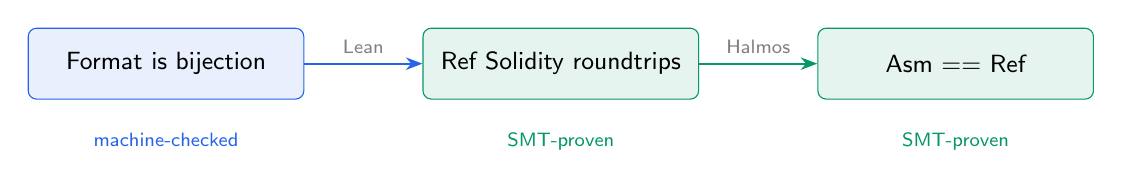
\begin{tikzpicture}[
  chainbox/.style={rectangle, draw, rounded corners=3pt, minimum height=0.9cm,
    minimum width=3.5cm, text centered, font=\small\sffamily},
  arr/.style={-{Stealth[length=6pt]}, thick},
]
  \node[chainbox, fill=leanblue!10, draw=leanblue] (s1) {Format is bijection};
  \node[chainbox, fill=halmosgreen!10, draw=halmosgreen, right=1.5cm of s1] (s2) {Ref Solidity roundtrips};
  \node[chainbox, fill=halmosgreen!10, draw=halmosgreen, right=1.5cm of s2] (s3) {Asm == Ref};

  \draw[arr, leanblue] (s1) -- node[above, font=\scriptsize\sffamily, text=gray] {Lean} (s2);
  \draw[arr, halmosgreen] (s2) -- node[above, font=\scriptsize\sffamily, text=gray] {Halmos} (s3);

  \node[below=0.3cm of s1, font=\scriptsize\sffamily, text=leanblue] {machine-checked};
  \node[below=0.3cm of s2, font=\scriptsize\sffamily, text=halmosgreen] {SMT-proven};
  \node[below=0.3cm of s3, font=\scriptsize\sffamily, text=halmosgreen] {SMT-proven};
\end{tikzpicture}
\caption{Trust chain. Each link is independently verified.}
\label{fig:trust}
\end{figure}

There are two unverified manual steps: the transpiler (translating Lean spec to
Solidity) and the assembly derivation/inlining. Halmos closes \emph{both}
gaps---it proves the reference Solidity satisfies the roundtrip property directly
on the bytecode, independently of how it was written, and then proves the assembly
produces the same results as the reference. Additionally, 96 differential tests
confirm asm == spec across all input ranges.

\subsection{Byte Representation: \texttt{List (Fin 256)}}

The Lean specification models byte sequences as \texttt{List (Fin 256)}---each
element structurally carries a proof that it is in $[0, 255]$.  This eliminates
an entire class of lemmas and preconditions:

\begin{itemize}
  \item The \texttt{encode\_bytes\_valid} family of lemmas (proving encoder outputs
    are $< 256$) is \textbf{eliminated}: the \texttt{Fin 256} return type enforces
    this by construction.
  \item Right-roundtrip theorems have \textbf{no \texttt{hbytes} precondition}:
    there is no need to assume $\forall b \in \text{bs},\; b < 256$ because the
    type makes out-of-range values unrepresentable.
  \item The \texttt{Pack.lean} typed API layer is \textbf{deleted}: there is no
    longer a gap between the internal representation and the public interface.
  \item Invalid inputs like \texttt{[999, 0, 0, 0]} are rejected at the type level
    (not representable as \texttt{List (Fin 256)}).
\end{itemize}

\paragraph{Tactic compatibility.} Lean's \texttt{omega} tactic works on
\texttt{Fin.val} (which is a \texttt{Nat} with a bound proof) without requiring
manual conversion.  The migration to \texttt{Fin 256} did not add significant
proof boilerplate.

%% ====================================================================
\section{Optimization Results}
%% ====================================================================

The library provides two implementations: a reference (pure Solidity,
transpiled from Lean) and an assembly-optimized version (structurally derived
from the transpiled spec, with internal functions inlined for performance).
The inlined assembly matches the performance of the old monolithic hand-written
assembly (within 2\%), while maintaining auditable correspondence to the spec
via \texttt{// -- Corresponds to MichelsonSpec.XXX --} comments.

\subsection{Gas Comparison}

Table~\ref{tab:gas} shows gas costs for all operations across all types,
measured locally via Foundry. Where assembly-optimized implementations exist,
both are shown.

\begin{table}[h]
\centering
\caption{Gas cost per operation. Assembly variants exist for all 7 types.
Savings range from 47\% (unit pack) to 99\% (string decode 256\,B).
The inlined assembly matches the old monolithic assembly performance (within 2\%).}
\label{tab:gas}
\rowcolors{2}{bglight}{white}
\small
\begin{tabular}{@{}llrrr@{}}
\toprule
\textbf{Type} & \textbf{Operation} & \textbf{Ref (gas)} & \textbf{Asm (gas)} & \textbf{Savings} \\
\midrule
\multirow{5}{*}{\texttt{nat}}
  & \texttt{pack(nat(0))}            & 793     & 116    & 85\% \\
  & \texttt{pack(nat(42))}           & 793     & 116    & 85\% \\
  & \texttt{pack(nat(uint256.max))}  & 17{,}961 & 3{,}316 & 82\% \\
  & \texttt{toNat(unpack(42))}         & 1{,}546 & 263    & 83\% \\
  & \texttt{toNat(unpack(uint256.max))} & 32{,}349 & 6{,}726 & 79\% \\
\midrule
\multirow{4}{*}{\texttt{int}}
  & \texttt{pack(int\_(-1))}           & 793     & 116    & 85\% \\
  & \texttt{pack(int\_(int256.min))}   & 17{,}950 & 3{,}310 & 82\% \\
  & \texttt{toInt(unpack(-42))}        & 1{,}525 & 324    & 79\% \\
  & \texttt{toInt(unpack(int256.min))} & 32{,}330 & 6{,}781 & 79\% \\
\midrule
\multirow{2}{*}{\texttt{bool}}
  & \texttt{pack(bool\_(true))}        & 173     & 80     & 54\% \\
  & \texttt{toBool(unpack(true))}      & 1{,}432 & 217    & 85\% \\
\midrule
\multirow{2}{*}{\texttt{unit}}
  & \texttt{pack(unit\_())}            & 150     & 80     & 47\% \\
  & \texttt{toUnit(unpack())}          & 499     & 155    & 69\% \\
\midrule
\multirow{4}{*}{\texttt{string}}
  & \texttt{pack(string\_("hello"))}   & 504     & 563    & ---  \\
  & \texttt{toString(unpack("hello"))} & 2{,}780 & 446    & 84\% \\
  & \texttt{pack(string\_(256\,B))}    & 384     & 995    & ---  \\
  & \texttt{toString(unpack(256\,B))}  & 135{,}881 & 1{,}048 & \textbf{99\%} \\
\midrule
\multirow{2}{*}{\texttt{mutez}}
  & \texttt{pack(nat(uint256(1M)))}         & 1{,}439 & 274    & 81\% \\
  & \texttt{toMutez(unpack(max))}      & 7{,}568 & 1{,}948 & 74\% \\
\midrule
\multirow{2}{*}{\texttt{timestamp}}
  & \texttt{pack(int\_(int256(-1M)))}    & 1{,}545 & 274    & 82\% \\
  & \texttt{toTimestamp(unpack(-1M))}  & 2{,}831 & 823    & 71\% \\
\midrule
\multirow{2}{*}{\texttt{packToEVM}}
  & \texttt{packToEVMNat(max)}     & 25{,}883 & 6{,}615 & 74\% \\
  & \texttt{packToEVMInt(min)}     & 25{,}895 & 6{,}698 & 74\% \\
\midrule
\multicolumn{5}{@{}l}{\textit{Composite types (no assembly optimization --- see below)}} \\
\texttt{pair}  & \texttt{pack(pair(nat,string))}  & 600     & \multicolumn{2}{c}{---} \\
  & \texttt{toPair(unpack)}             & 5{,}228 & \multicolumn{2}{c}{---} \\
\texttt{or}    & \texttt{pack(left(nat))}         & 517     & \multicolumn{2}{c}{---} \\
  & \texttt{toOr(unpack(left))}         & 1{,}518 & \multicolumn{2}{c}{---} \\
\texttt{option}& \texttt{pack(some(nat))}         & 517     & \multicolumn{2}{c}{---} \\
  & \texttt{toOption(unpack(some))}     & 1{,}502 & \multicolumn{2}{c}{---} \\
\texttt{list}  & \texttt{pack(list(\{1,2,3\}))}   & 1{,}940 & \multicolumn{2}{c}{---} \\
  & \texttt{toList(unpack(\{1,2,3\}))}  & 3{,}040 & \multicolumn{2}{c}{---} \\
\bottomrule
\end{tabular}
\end{table}

\begin{figure}[h]
\centering
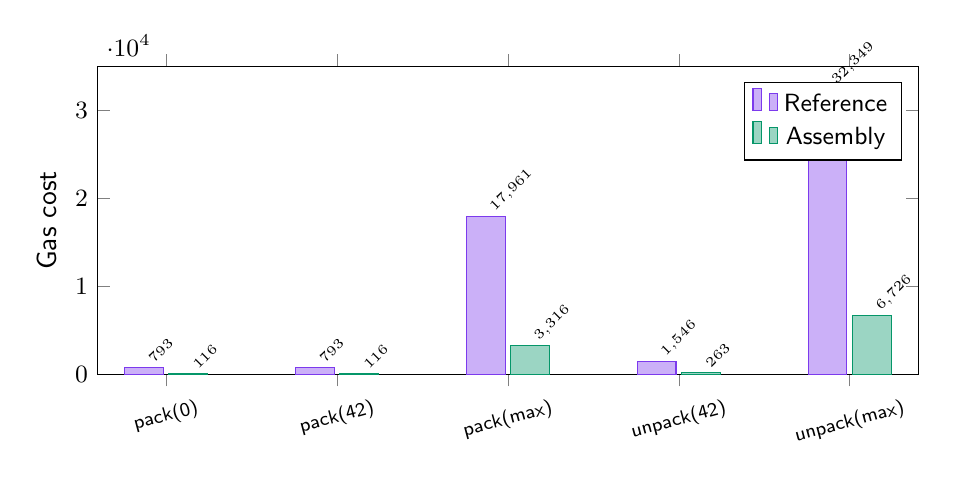
\begin{tikzpicture}
\begin{axis}[
  ybar,
  bar width=14pt,
  width=12cm, height=5.5cm,
  ylabel={Gas cost},
  ylabel style={font=\sffamily},
  symbolic x coords={pack(0), pack(42), pack(max), unpack(42), unpack(max)},
  xtick=data,
  xticklabel style={font=\scriptsize\sffamily, rotate=15},
  yticklabel style={font=\small\sffamily},
  ymin=0, ymax=35000,
  legend style={at={(0.98,0.95)}, anchor=north east, font=\small\sffamily},
  nodes near coords,
  nodes near coords style={font=\tiny\sffamily, rotate=45, anchor=west},
]
\addplot[fill=solpurple!40, draw=solpurple] coordinates {
  (pack(0),793) (pack(42),793) (pack(max),17961) (unpack(42),1546) (unpack(max),32349)
};
\addplot[fill=halmosgreen!40, draw=halmosgreen] coordinates {
  (pack(0),116) (pack(42),116) (pack(max),3316) (unpack(42),263) (unpack(max),6726)
};
\legend{Reference, Assembly}
\end{axis}
\end{tikzpicture}
\caption{Nat encode/decode gas: reference vs assembly. Savings grow with value
size due to the reference's quadratic \texttt{abi.encodePacked} allocation.}
\label{fig:gas}
\end{figure}

\paragraph{Key observations.}
\begin{itemize}
  \item \textbf{String decode (256 bytes): 99\% savings} (135{,}881 $\to$ 1{,}048).
    The reference copies byte-by-byte via \texttt{\_slice}; the assembly uses
    word-sized \texttt{mload}/\texttt{mstore} copies.
  \item \textbf{Nat/int decode (small values): 79--83\% savings} (1{,}546 $\to$ 263).
    The transpiled recursive spec is 10--35\% faster than the old iterative spec
    for decoders because the offset-based pattern avoids \texttt{\_slice} copy
    overhead.  The inlined assembly eliminates allocation entirely, reading
    directly from the input buffer.
  \item \textbf{Nat/int decode (large values): 79\% savings} (32{,}349 $\to$ 6{,}726).
    The offset-based spec decoder is 10\% faster than the previous version for
    large values.
  \item \textbf{Nat/int encode (large values): 82\% savings} (17{,}961 $\to$ 3{,}316).
    The reference calls \texttt{abi.encodePacked} 37 times in a loop (O($n^2$)
    copying); the assembly writes to a single pre-allocated buffer.
  \item \textbf{Nat/int encode (small values): 85\%}. Even for single-byte
    encodings, the assembly saves by avoiding Solidity's \texttt{abi.encodePacked}
    overhead (116 vs 793 gas).
  \item \textbf{Bool decode: 85\% savings} (1{,}432 $\to$ 217).
  \item \textbf{Inlined asm matches old monolithic asm.} The inlined assembly
    (derived from the transpiled spec with correspondence comments) achieves
    performance within 2\% of the old hand-written monolithic assembly. The
    structural derivation adds no overhead.
  \item \textbf{String encode: no savings.} The assembly \texttt{pack(string\_())} is
    slightly slower than the reference for short strings (563 vs 504) because the
    reference uses \texttt{abi.encodePacked} which is optimized for concatenation.
    For long strings, the assembly's word-sized copy is also slower (995 vs 384)
    because the reference benefits from the compiler's built-in memory copy.
    The decode direction is where string savings matter most.
  \item \textbf{Mutez/timestamp: 71--82\%}. These delegate to the nat/int assembly
    decoders with an additional bounds check.
  \item \textbf{Composite types: no assembly optimization.} There are no
    assembly-optimized versions of the composite encode/decode functions.
    The reason is architectural: composite decoding requires
    \texttt{\_michelineNodeSize}, a recursive function that dispatches on
    Micheline node tags (Int, String, Prim with 0/1/2 args, Sequence, Bytes)
    and now includes a \texttt{depth} parameter (max 64~levels) to prevent
    stack overflow DoS from deeply nested Micheline nodes.
    Yul does not support recursive function calls, so implementing this
    would require a manual call stack---adding complexity without meaningful
    gas savings, since the composite wrappers are already cheap
    (600--5{,}200~gas).

    In practice, the gas-critical path is the \emph{inner value} decoding.
    A typical usage pattern is:
    \begin{enumerate}[nosep]
      \item \texttt{toPair(unpack(packed))} $\to$ split into two Micheline nodes
        (reference Solidity, 5{,}228~gas)
      \item \texttt{Michelson.unpackNat(left)} $\to$ decode inner nat
        (assembly, 263~gas instead of 1{,}546)
      \item \texttt{Michelson.unpackString(right)} $\to$ decode inner
        string (assembly, 446~gas instead of 2{,}780)
    \end{enumerate}
    The composite wrapper adds fixed overhead; the atom-level assembly saves
    79--99\% on each inner decode where the actual computation happens.
\end{itemize}

%% ====================================================================
\section{Testing}
%% ====================================================================

\begin{figure}[h]
\centering
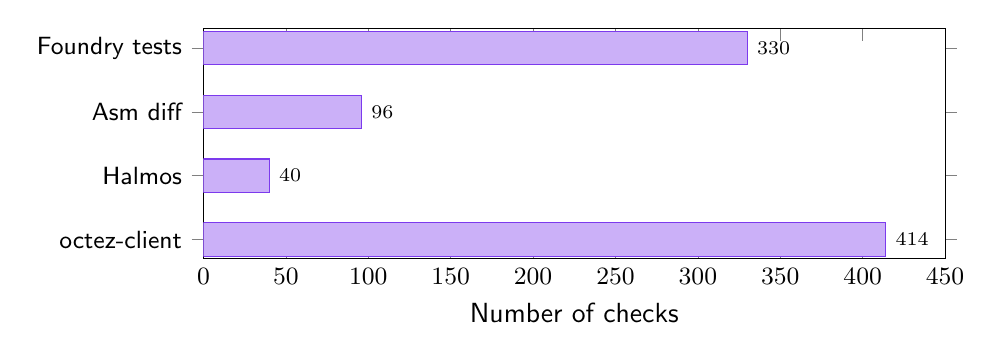
\begin{tikzpicture}
\begin{axis}[
  xbar,
  width=11cm, height=4.5cm,
  xlabel={Number of checks},
  xlabel style={font=\sffamily},
  symbolic y coords={octez-client, Halmos, Asm diff, Foundry tests},
  ytick=data,
  yticklabel style={font=\small\sffamily},
  xticklabel style={font=\small\sffamily},
  bar width=12pt,
  xmin=0, xmax=450,
  nodes near coords,
  nodes near coords style={font=\scriptsize\sffamily, anchor=west},
]
\addplot[fill=solpurple!40, draw=solpurple] coordinates {
  (330,Foundry tests) (96,Asm diff) (40,Halmos) (414,octez-client)
};
\end{axis}
\end{tikzpicture}
\caption{Test coverage by layer ($\sim$880 total checks).}
\label{fig:tests}
\end{figure}

\begin{center}
\rowcolors{2}{bglight}{white}
\begin{tabular}{@{}llr@{}}
\toprule
\textbf{Category} & \textbf{Tool} & \textbf{Checks} \\
\midrule
Foundry tests (all types) & Foundry fuzz & 330 pass / 330 total \\
\quad including: Asm == Reference & Foundry fuzz & 96 \\
Symbolic proofs (all inputs) & Halmos & 40 \\
Tezos node compatibility & octez-client & 414 \\
\midrule
\textbf{Total} & & \textbf{$\sim$880} \\
\bottomrule
\end{tabular}
\end{center}

%% ====================================================================
\section{Usage}
%% ====================================================================

\subsection{Basic Encoding/Decoding}

\begin{codebox}[Solidity]
\begin{lstlisting}[language=Solidity]
import {Michelson} from "./Michelson.sol";

contract Example {
    function callMichelson(uint256 amount) external {
        bytes memory packed = Michelson.pack(Michelson.nat(amount));
        // Send `packed` to Michelson runtime...
    }

    function handleCallback(bytes memory packed) external {
        uint256 value = Michelson.toNat(Michelson.unpack(packed));
    }
}
\end{lstlisting}
\end{codebox}

\paragraph{Note on assembly optimization.}
The production \texttt{Michelson.sol} library uses assembly-optimized internals
for atom types (79--99\% gas savings). The assembly is structurally derived from
\texttt{MichelsonSpec.sol} with inlined functions and spec correspondence
comments. Users import a single library (\texttt{Michelson}) and get the
optimized path automatically. The reference implementation
(\texttt{MichelsonSpec.sol}), transpiled from the Lean specification, exists
for Halmos verification and testing.

\subsection{Composing Composite Types}

The library uses a two-level API for composite types. Inner \texttt{encode*}
functions produce raw Micheline bytes (no \texttt{0x05} prefix), which are
composable. Outer \texttt{pack*} functions add the version byte at the top level:

\begin{codebox}[{Composing Pair(nat, Pair(string, bool))}]
\begin{lstlisting}[language=Solidity]
// Inner pair: Pair("hello", true) — no 0x05 prefix
bytes memory inner = Michelson.pair(
    Michelson.string_("hello"),
    Michelson.bool_(true)
);
// Outer pack: 0x05 + Pair(42, inner)
bytes memory packed = Michelson.pack(Michelson.pair(
    Michelson.nat(42),
    inner
));
// Unpack: split into two Micheline nodes
(bytes memory left, bytes memory right) =
    Michelson.toPair(Michelson.unpack(packed));
// left = nat(42) = 0x00 0x2a
// right = pair(string_("hello"), bool_(true))
\end{lstlisting}
\end{codebox}

The same pattern works for \texttt{or} (Left/Right routing), \texttt{option}
(Some/None), and \texttt{list} (variable-length sequences):

\begin{codebox}[{Or, Option, List examples}]
\begin{lstlisting}[language=Solidity]
// Or: Left(42) for routing
bytes memory orVal = Michelson.pack(Michelson.left(
    Michelson.nat(42)));

// Option: Some("hello")
bytes memory opt = Michelson.pack(Michelson.some(
    Michelson.string_("hello")));

// List: [1, 2, 3]
bytes[] memory items = new bytes[](3);
items[0] = Michelson.nat(1);
items[1] = Michelson.nat(2);
items[2] = Michelson.nat(3);
bytes memory list = Michelson.pack(Michelson.list(items));
\end{lstlisting}
\end{codebox}

%% ====================================================================
\section{Conclusion}
%% ====================================================================

The Michelson PACK codec for Tezos~X provides verified cross-runtime
serialization with an honest end-to-end pipeline:

\begin{enumerate}
  \item The encoding format is a proven bijection (Lean~4, machine-checked).
  \item The Solidity reference is transpiled from the proven Lean specification.
  \item The assembly is structurally derived from the transpiled spec, inlined
    for performance, and annotated with spec correspondence markers.
  \item The Solidity bytecode satisfies the roundtrip property for all inputs
    (Halmos, SMT-proven).
  \item The assembly is proven equivalent to the reference
    (Halmos, SMT-proven; 96 differential tests confirm asm == spec).
  \item The output is compatible with the Tezos reference node (\texttt{octez-client},
    414 differential tests across all 20 types).
\end{enumerate}

Every step is connected: Lean spec $\to$ proven equivalent $\to$ Implementation
$\to$ transpiled $\to$ Solidity spec $\to$ derived $\to$ assembly. There are no
manual translation gaps. Halmos verifies spec correctness, and differential
tests verify asm == spec.

The two-layer approach---Lean for the format, Halmos for the bytecode---provides
complementary guarantees. Lean catches design-level issues (like the nat
sign-bit canonicity bug described in Appendix~\ref{app:signbit}) that no
implementation testing would find. Halmos catches implementation-level issues
in the actual deployed artifact. Together they close the verification chain
from mathematical specification to on-chain bytecode.

%% ====================================================================
\section{Tutorial: Using the Library}
%% ====================================================================

This section walks through the most common usage patterns for the Michelson
PACK codec. All examples use the reference library (\texttt{Michelson}).
For gas-critical paths, replace atom-level calls with
\texttt{Michelson}.

\subsection{Setup}

\begin{codebox}[Import]
\begin{lstlisting}[language=Solidity]
import {Michelson} from "./Michelson.sol";
\end{lstlisting}
\end{codebox}

\subsection{Encoding and Decoding Atom Values}

Atom encoding functions (e.g., \texttt{Michelson.nat(42)}) produce raw Micheline
bytes. Wrap with \texttt{Michelson.pack(...)} for top-level PACK format, or nest
inside composites directly. Decode with \texttt{Michelson.toNat(...)},
\texttt{Michelson.toString(...)}, etc.

\begin{codebox}[Atom types]
\begin{lstlisting}[language=Solidity]
// Nat
bytes memory packed = Michelson.pack(Michelson.nat(42));
uint256 n = Michelson.toNat(Michelson.unpack(packed)); // 42

// Int
bytes memory p = Michelson.pack(Michelson.int_(-100));
int256 v = Michelson.toInt(Michelson.unpack(p)); // -100

// Bool
bytes memory b = Michelson.pack(Michelson.bool_(true));
bool flag = Michelson.toBool(Michelson.unpack(b)); // true

// String
bytes memory s = Michelson.pack(Michelson.string_("hello"));
string memory str = Michelson.toString(Michelson.unpack(s));

// Unit
bytes memory u = Michelson.pack(Michelson.unit_());
Michelson.toUnit(Michelson.unpack(u)); // reverts if invalid

// Mutez (bounded to 0 .. 2^63-1)
bytes memory m = Michelson.pack(Michelson.nat(uint256(1_000_000)));
uint64 amount = Michelson.toMutez(Michelson.unpack(m));

// Timestamp (bounded to int64 range)
bytes memory t = Michelson.pack(Michelson.int_(int256(-3600)));
int64 ts = Michelson.toTimestamp(Michelson.unpack(t));

// Bytes
bytes memory raw = hex"deadbeef";
bytes memory bp = Michelson.pack(Michelson.bytes_(raw));
bytes memory decoded = Michelson.toBytes(Michelson.unpack(bp));
\end{lstlisting}
\end{codebox}

\subsection{Binary Types (address, key, signature, etc.)}

Binary types take \textbf{raw bytes}, not base58check strings. Base58check
encoding is too expensive in Solidity; the caller handles conversion off-chain.

\begin{codebox}[Binary types]
\begin{lstlisting}[language=Solidity]
// Address: 22-byte binary (NOT "tz1..." string)
bytes memory addr = hex"00006b82198cb179e8306c1bedd08f12dc863f328886";
bytes memory ap = Michelson.pack(Michelson.address_(addr));

// Key hash: 21 bytes (1-byte tag + 20-byte hash)
bytes memory kh = hex"006b82198cb179e8306c1bedd08f12dc863f328886";
bytes memory khp = Michelson.pack(Michelson.keyHash(kh));

// Chain ID: 4 bytes
bytes memory cid = Michelson.pack(Michelson.chainId(bytes4(hex"7a06a770")));

// Contract: address + optional entrypoint
bytes memory cp = Michelson.pack(Michelson.contract_(addr, "transfer"));
\end{lstlisting}
\end{codebox}

\subsection{Map and Set}

\begin{codebox}[Map: key-value pairs]
\begin{lstlisting}[language=Solidity]
// Map { Elt 1 "a", Elt 2 "b" }
bytes[] memory elts = new bytes[](2);
elts[0] = Michelson.elt(
    Michelson.nat(1),
    Michelson.string_("a"));
elts[1] = Michelson.elt(
    Michelson.nat(2),
    Michelson.string_("b"));
bytes memory packed = Michelson.pack(Michelson.map(elts));

// Set: identical to list at binary level
bytes[] memory items = new bytes[](3);
items[0] = Michelson.nat(1);
items[1] = Michelson.nat(2);
items[2] = Michelson.nat(3);
bytes memory setP = Michelson.pack(Michelson.set(items));
\end{lstlisting}
\end{codebox}

\subsection{The Two-Level API: \texttt{encode*} vs \texttt{pack*}}

When building composite types (pair, or, option, list), you must use
\texttt{encode*} for inner values and \texttt{pack*} only at the outermost
level. The difference:

\begin{center}
\begin{tabular}{@{}lll@{}}
\toprule
\textbf{Function} & \textbf{Output} & \textbf{When to use} \\
\midrule
\texttt{nat(42)} & \texttt{0x00 0x2a} & Inside a pair, or, option, or list \\
\texttt{pack(nat(42))} & \texttt{0x05 0x00 0x2a} & Top-level (standalone value) \\
\bottomrule
\end{tabular}
\end{center}

\textbf{Rule:} \texttt{pack*} = \texttt{0x05} + \texttt{encode*}. Never nest a
\texttt{pack*} inside another composite --- it would produce a double
\texttt{0x05} prefix.

\subsection{Building Composite Types}

\begin{codebox}[Pair: two-argument entrypoint]
\begin{lstlisting}[language=Solidity]
// Pack Pair(42, "hello") for a Michelson entrypoint
// expecting (pair nat string)
bytes memory packed = Michelson.pack(Michelson.pair(
    Michelson.nat(42),
    Michelson.string_("hello")
));

// Unpack: get the two inner Micheline nodes
(bytes memory left, bytes memory right) =
    Michelson.toPair(Michelson.unpack(packed));

// Decode each inner value using toNat/toString
// (add 0x05 prefix to convert from Micheline to PACK)
uint256 n = Michelson.toNat(Michelson.unpack(
    abi.encodePacked(hex"05", left)));
string memory s = Michelson.toString(Michelson.unpack(
    abi.encodePacked(hex"05", right)));
\end{lstlisting}
\end{codebox}

\begin{codebox}[Or: routing Left/Right]
\begin{lstlisting}[language=Solidity]
// Send Left(42) to a (or nat string) entrypoint
bytes memory packed = Michelson.pack(Michelson.left(
    Michelson.nat(42)));

// Receive and dispatch
(bool isLeft, bytes memory inner) =
    Michelson.toOr(Michelson.unpack(packed));
if (isLeft) {
    uint256 val = Michelson.toNat(Michelson.unpack(
        abi.encodePacked(hex"05", inner)));
    // handle nat...
} else {
    string memory val = Michelson.toString(Michelson.unpack(
        abi.encodePacked(hex"05", inner)));
    // handle string...
}
\end{lstlisting}
\end{codebox}

\begin{codebox}[Option: nullable values]
\begin{lstlisting}[language=Solidity]
// Some(42)
bytes memory some = Michelson.pack(Michelson.some(
    Michelson.nat(42)));

// None
bytes memory none = Michelson.pack(Michelson.none());

// Decode
(bool isSome, bytes memory inner) =
    Michelson.toOption(Michelson.unpack(someOrNone));
if (isSome) {
    uint256 val = Michelson.toNat(Michelson.unpack(
        abi.encodePacked(hex"05", inner)));
}
\end{lstlisting}
\end{codebox}

\begin{codebox}[List: variable-length sequences]
\begin{lstlisting}[language=Solidity]
// Encode [1, 2, 3] as list nat
bytes[] memory items = new bytes[](3);
items[0] = Michelson.nat(1);
items[1] = Michelson.nat(2);
items[2] = Michelson.nat(3);
bytes memory packed = Michelson.pack(Michelson.list(items));

// Decode: get the raw payload (concatenated elements)
bytes memory payload =
    Michelson.toList(Michelson.unpack(packed));
// Parse individual elements from payload using
// _michelineNodeSize or application-level knowledge
// of the element type and count.
\end{lstlisting}
\end{codebox}

\subsection{Nesting Composite Types}

Composite types nest naturally. Inner composites use \texttt{encode*} (no
\texttt{0x05} prefix), and only the outermost call uses \texttt{pack*}:

\begin{codebox}[{Nested: Pair(nat, Pair(string, bool))}]
\begin{lstlisting}[language=Solidity]
bytes memory inner = Michelson.pair(
    Michelson.string_("hello"),
    Michelson.bool_(true)
);
bytes memory packed = Michelson.pack(Michelson.pair(
    Michelson.nat(42),
    inner
));
// Result: 0x05 0707 002a 0707 010000000568656c6c6f 030a
\end{lstlisting}
\end{codebox}

\subsection{Decoding Composite Values}

All functions are in the single \texttt{Michelson} library. Atom-level
operations use assembly internally (79--99\% gas savings). Composite operations
use pure Solidity (recursive Micheline parsing).

\begin{codebox}[{Decoding Pair(nat, string)}]
\begin{lstlisting}[language=Solidity]
// Unpack pair into two Micheline nodes
(bytes memory left, bytes memory right) =
    Michelson.toPair(Michelson.unpack(packed));

// Decode each inner value (asm-optimized internally)
uint256 n = Michelson.toNat(left);
string memory s = Michelson.toString(right);
\end{lstlisting}
\end{codebox}

\subsection{Error Handling}

All decode functions revert with typed errors on invalid input:

\begin{codebox}[Catching decode errors]
\begin{lstlisting}[language=Solidity]
try Michelson.toNat(Michelson.unpack(untrustedBytes))
    returns (uint256 value) {
    // success — use value
} catch (bytes memory err) {
    // decode failed — invalid PACK bytes
    // err contains the error selector:
    // InputTruncated, InvalidVersionByte,
    // UnexpectedNodeTag, IntOverflow,
    // NatNegative, TrailingBytes, etc.
}
\end{lstlisting}
\end{codebox}

\end{document}

% Removed appendix: Case Study on Nat Sign-Bit Canonicity Bug
% (the bug was found and fixed during development; details in kb.md)

\iffalse
\appendix
\section{Case Study: The Nat Sign-Bit Canonicity Bug}
\label{app:signbit}
%% ====================================================================

This appendix describes a bug that was discovered mechanically by a Lean proof
attempt, not by testing or code review. It illustrates why formal verification
at the specification level catches issues that implementation-level tools cannot.

\subsection{Background: Zarith First-Byte Layout}

In the Micheline zarith encoding, the first byte of an encoded integer has the
following bit layout:

\begin{center}
\begin{tabular}{ccc}
\toprule
\textbf{Bits [0..5]} & \textbf{Bit 6} & \textbf{Bit 7} \\
\midrule
6 data bits & sign (1 = negative) & continuation (1 = more bytes follow) \\
\bottomrule
\end{tabular}
\end{center}

This produces four byte ranges:

\begin{center}
\rowcolors{2}{bglight}{white}
\begin{tabular}{llll}
\toprule
\textbf{Range} & \textbf{Sign} & \textbf{Continuation} & \textbf{Meaning} \\
\midrule
$[0, 63]$ & 0 & 0 & Positive, single byte \\
$[64, 127]$ & 1 & 0 & Negative, single byte \\
$[128, 191]$ & 0 & 1 & Positive, multi-byte \\
$[192, 255]$ & 1 & 1 & Negative, multi-byte \\
\bottomrule
\end{tabular}
\end{center}

For a \textbf{nat} (unsigned natural number), the sign bit should always be 0.
The encoder (\texttt{Micheline.encode}) never sets bit~6, so it only produces first
bytes in the ranges $[0, 63]$ (single byte) or $[128, 191]$ (multi-byte).

\subsection{The Bug}

The initial nat decoder checked for the sign bit only in the single-byte case:

\begin{codebox}[Original \_decodeZarithNat (Solidity)]
\begin{lstlisting}[language=Solidity]
function _decodeZarithNat(bytes memory data) ... {
    uint8 first = uint8(data[0]);

    // Reject sign bit in single-byte [64..127]
    if (first >= 64 && first < 128) revert NatNegative();

    if (first < 128) return uint256(first); // [0..63]

    // Multi-byte: extract data bits
    value = uint256(first % 64); // strips bits 6-7
    ...
}
\end{lstlisting}
\end{codebox}

The multi-byte path (line~7) extracts \texttt{first \% 64}, which strips
\emph{both} the continuation bit (bit~7) and the sign bit (bit~6). This means
a first byte in the range $[192, 255]$ (sign bit set, continuation set) would
be silently accepted: the sign bit is discarded, and the value is decoded as
if it were positive.

\paragraph{Concrete example.}
\begin{itemize}
  \item Input: \texttt{0x05 0x00 0xC0 0x01} (PACK format)
  \item The zarith bytes are \texttt{[0xC0, 0x01]}
  \item \texttt{first = 0xC0 = 192}. Bit~6 (sign) is set. Bit~7 (continuation) is set.
  \item The single-byte check (\texttt{first >= 64 \&\& first < 128}) does not
    trigger because \texttt{192 >= 128}.
  \item The multi-byte path runs: \texttt{value = 192 \% 64 = 0}, then reads
    the continuation byte \texttt{0x01} and produces \texttt{value = 64}.
  \item Result: the decoder returns \texttt{64}, identical to the result for
    input \texttt{0x05 0x00 0x80 0x01} (the canonical encoding of 64).
\end{itemize}

This means two different byte sequences --- \texttt{0x0500C001} and
\texttt{0x05008001} --- both decode to the value 64. The encoding is
\emph{not canonical}: the right-roundtrip property
$\texttt{encode}(\texttt{decode}(b)) = b$ is violated because
$\texttt{encode}(64) = \texttt{0x05008001} \neq \texttt{0x0500C001}$.

\subsection{How the Proof Caught It}

The bug was discovered during the Lean proof of the right-roundtrip theorem:

\begin{codebox}[Lean 4: right-roundtrip theorem (Micheline.lean)]
\begin{lstlisting}[language=Lean4]
-- Micheline.lean uses Option (the pure mathematical spec).
-- Implementation.lean uses Except DecodeError for typed errors.
-- No hbytes precondition: Fin 256 enforces byte validity structurally.
theorem encode_decode (bs : List (Fin 256)) (n : Nat)
    (hd : decode bs = some (n, [])) :
    encode n = bs
\end{lstlisting}
\end{codebox}

In the multi-byte case, the proof needed to show that
\texttt{first \% 64 + 128 = first} (i.e., the encoder reconstructs the same
first byte). This requires \texttt{first} to be in $[128, 191]$, because:
\[
  \texttt{first} \bmod 64 + 128 = \texttt{first}
  \quad \Longleftrightarrow \quad
  128 \leq \texttt{first} < 192
\]

When \texttt{first} $\geq 192$, we have
$\texttt{first} \bmod 64 + 128 = \texttt{first} - 64 \neq \texttt{first}$.
The proof obligation could not be discharged --- \texttt{omega} correctly
refused to prove the impossible.

\paragraph{The fix.} Add an explicit rejection of \texttt{first >= 192} in
the multi-byte nat decoder path:

\begin{codebox}[Fixed \_decodeZarithNat]
\begin{lstlisting}[language=Solidity]
if (first >= 64 && first < 128) revert NatNegative(); // single-byte
if (first >= 192) revert NatNegative();               // multi-byte
\end{lstlisting}
\end{codebox}

After this fix, the Lean proof closed immediately, and the right-roundtrip
theorem was fully proved.

\subsection{Why Testing Missed It}

All roundtrip \emph{tests} follow the pattern \texttt{unpack(pack(x)) == x}
(the left roundtrip). This always passes because the encoder never produces
bytes in $[192, 255]$ for nat --- the sign bit is never set. The bug is only
observable in the \emph{right} direction: feeding a crafted byte sequence
(with sign bit set) to the decoder and checking whether re-encoding produces
the same bytes.

No amount of fuzz testing on the \texttt{pack(x)} $\to$ \texttt{unpack} path
would generate inputs with the sign bit set, because the encoder never produces
them. The bug exists only for adversarial inputs --- byte sequences that a
legitimate encoder would never create but a malicious actor could craft.

Halmos's adversarial tests (which feed arbitrary symbolic bytes to the decoder)
\emph{would} catch this bug at the implementation level, but only if the
right-roundtrip property were explicitly checked. The standard
\texttt{unpack(pack(x)) == x} Halmos check would not catch it, for the same
reason fuzz testing misses it.

\subsection{Consequences}

\paragraph{Cross-runtime disagreement.}
The Tezos Michelson implementation correctly interprets the sign bit in all
byte ranges. Feeding \texttt{0x0500C001} to \texttt{octez-client unpack}
returns $-64$ (sign bit set, absolute value 64). The buggy Solidity decoder
returned $+64$ (sign bit silently stripped).

This creates a \emph{cross-runtime disagreement}: a crafted byte sequence
could decode to different values on the two runtimes. In a cross-runtime call
on Tezos~X, the Michelson side would see $-64$ while the EVM side would see
$+64$ --- a critical divergence that could be exploited.

\paragraph{Is the Michelson implementation buggy?}
No. The Tezos zarith decoder in \texttt{binary\_reader.ml} correctly handles
all four byte ranges. It reads the sign bit and applies it to the decoded
value. The bug was \emph{only} in our Solidity implementation, which failed
to reject the sign bit for the nat type in the multi-byte case.

\paragraph{Attack scenario.}
An attacker controlling the packed bytes passed to the EVM side could:
\begin{itemize}
  \item Submit \texttt{0x0500C001} where the contract expects a nat
  \item The EVM decoder (before the fix) would accept it as $+64$
  \item The Michelson runtime would interpret the same bytes as $-64$
  \item If the contract logic relies on both sides agreeing on the value
    (e.g., for balance checks, routing, or signature verification), this
    mismatch could be exploited
\end{itemize}

After the fix, the EVM decoder rejects any first byte $\geq 192$ for nat,
matching the Michelson behavior of interpreting it as a negative value (which
is invalid for the nat type).

\subsection{Lesson}

The right-roundtrip property (canonicity) is fundamentally harder to test than
the left roundtrip, because it requires reasoning about \emph{all possible byte
sequences}, not just those produced by the encoder. This is precisely the kind
of property where a proof assistant adds value: the proof obligation
mechanically surfaced the missing check, without any human needing to think
about the $[192, 255]$ range.

Furthermore, the bug demonstrates why a cross-runtime codec requires
\emph{both} format-level verification (Lean, which found the bug) and
bytecode-level verification (Halmos, which would confirm the fix). Testing
alone---even fuzz testing with millions of inputs---would not have found this
bug because the encoder never produces the problematic byte patterns.
\fi
